\documentclass[]{IEEEtran}

\title{Exploiting Automatic Abstraction and the FMI Standard to build Cycle-accurate Virtual Platforms from 
Heterogeneous IPs}
\author{Vladislav Bragoi - VR436747}

\usepackage{graphicx}
\usepackage[utf8]{inputenc}
\usepackage[italian]{babel}
\usepackage{booktabs}
\usepackage{float}
\usepackage{caption}
\usepackage{minted}
\usepackage{url}
\usepackage{tikz}
\usetikzlibrary{shapes,arrows}
\newcommand{\var}[1]{\textit{#1}}
\newcommand{\code}[1]{\texttt{#1}}
\renewcommand{\arraystretch}{1.2}
\begin{document}
\maketitle

\begin{abstract}
In questo documento vengono descritte le principali fasi di creazione dei pacchetti FMU, al fine di poter co-simulare un 
sistema costituito da IP eterogenei.

\end{abstract}

\section{Introduzione}
In questo progetto si vogliono provare e analizzare i principali vantaggi e le potenzialit\`a introdotte dallo standard
FMI, andando a toccare con mano una possibile implementazione di un modulo rispettando lo standard, e la sua integrazione 
in un sistema pi\`u complesso costituito di elementi eterogenei. 

\section{Background}
Il Functional Mockup Interface (FMI)\cite{FMI} è un protocollo che standardizza la comunicazione tra modelli ciberfisici 
eterogenei scritti in diversi linguaggi di programmazione, supportandone la co-simulazione attraverso la definizione di
un'interfaccia del singolo modello definita in un file xml e la cui funzionalit\`a \`e interamente espressa da un 
sorgente o compilato in codice C.
Il singolo elemento che implementa tale protocollo è detto Functional Mockup Unit (FMU).

\section{Metodologia applicata}
Poich\'e questo \`e un tutorial che andava semplicemente completato, \`e stato sufficiente completare le parti mancanti 
nei sorgenti C++ del modulo \emph{gain} e integrarne la funzionalit\`a all'interno del coordinatore definito nel file 
\code{coordinator.py}.
Di seguito i dettagli.

\subsection{GAIN}
Il modulo gain da specifica deve moltiplicare per 10 (costante \var{GAIN\_VALUE}) il valore che gli arriva in ingresso. 
Per fare ci\`o, oltre ad aggiungere la variabile \mintinline{C}{result} nel file header del modulo, che dev'essere 
inoltre definita anche nel file \code{modelDescription.xml} come porta di output e inizializzata a 0, \`e stato 
necessario modificarne il comportamento come segue:
\begin{itemize}
    \item se \var{data\_rdy} \`e a true, il valore del dato dev'essere moltiplicato per la costante \var{GAIN\_VALUE} e
            memorizzato nella variabile \mintinline{C}{result} definita precedentemente,
    \item \mintinline{C}{result} deve essere settato a 0 altrimenti.
\end{itemize}
Compilando il modulo con il comando \mintinline{shell}{cmake} viene generato il file \code{.so} da utilizzare nella 
successiva generazione dell'archivio \code{.fmu}. 

\subsection{Generazione delle FMU}
Per generare gli archivi \code{.fmu} è sufficiente utilizzare il comando \mintinline{shell}{make} una volta che 
ci si \`e posizionati nella directory contenente, come gi\`a detto precedentemente, i file \code{.xml} dell'interfaccia 
del modulo appunto e \code{.so} del codice binario che ne racchiude la funzionalit\`a.
I makefile che accompagnano ciascun modulo contengono al loro interno i comandi necessari per la generazione delle 
corrispondenti functional mockup unit, a partire da codice Verilog-A (analog) per il modulo \emph{Accelerometer} e
Verilog per il modulo \emph{m6502} e il modulo \emph{memory}.
Questi comandi vengono riportati in figura \ref{fig:schema}, e nello specifico sono:
\begin{itemize}
    \item \mintinline{shell}{verilog2hif}, per tradurre il codice Verilog nel formato HIF utilizzato dall'insieme dei 
    tool che costituiscono la HIFSuite,
    \item \mintinline{shell}{analyst}, per generare modelli HIF a eventi discreti a partire da un design analogico quale
        quello dell'Accelerometer,
    \item \mintinline{shell}{ddt}, per una conversione dei tipi di dato definiti nel modulo con quelli nativi del codice C,
    \item \mintinline{shell}{a2tool}, per una traduzione in C++/SystemC a partire dalla rappresentazione HIF-RTL,
    \item \mintinline{shell}{hif2vp}, per la generazione del documento xml che descrive il modulo, da inserire 
        nell'archivio \code{.fmu}.
\end{itemize}

\subsection{Coordinatore}
Il coordinatore \`e l'elemento tramite il quale riusciamo a simulare l'intero sistema sfruttando lo standard FMI.
Essendo scritto in Python, il framework PyFMI\cite{PyFMI} \`e di riferimento per implementare le funzionalit\`a del 
master in modo da poter caricare le varie FMU e farle interagire tra loro.
La sua implementazione \`e definita nel file \code{coordinator.py} ed \`e stata aggiornata per includere la
funzionalit\`a aggiunta del modulo gain.

\begin{figure*}[h]
    \centering
    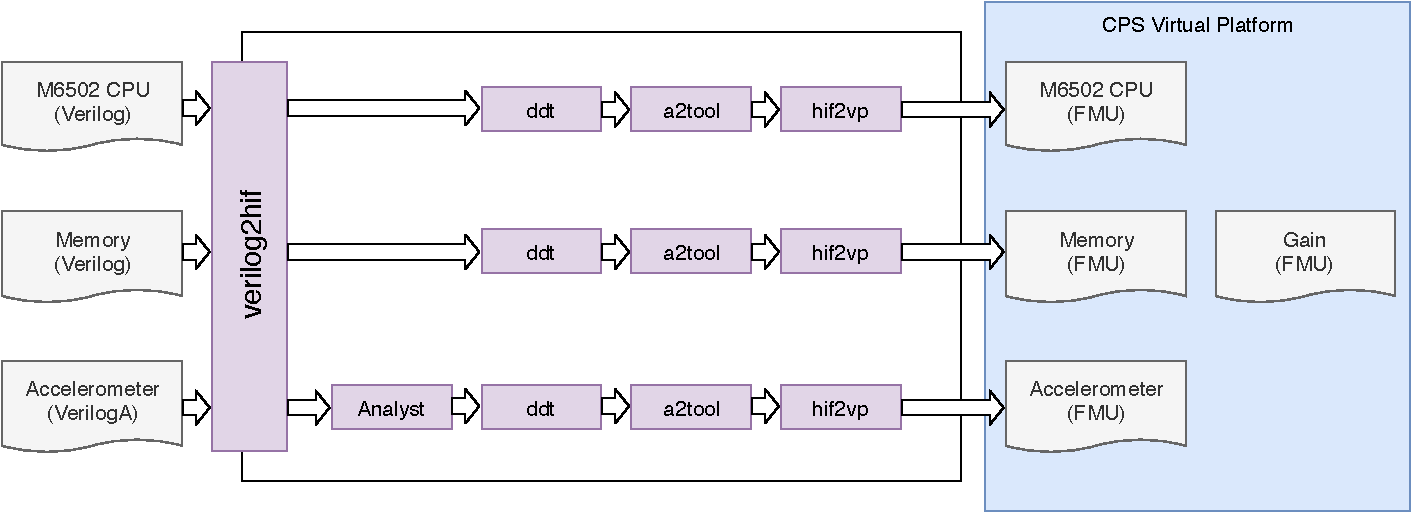
\includegraphics[width=0.7\textwidth]{figures/schema}
	\caption{Comandi necessari per generare i file \code{.fmu} a partire dai vari sorgenti}
	\label{fig:schema}
\end{figure*}

\begin{figure*}[h]
    \centering
    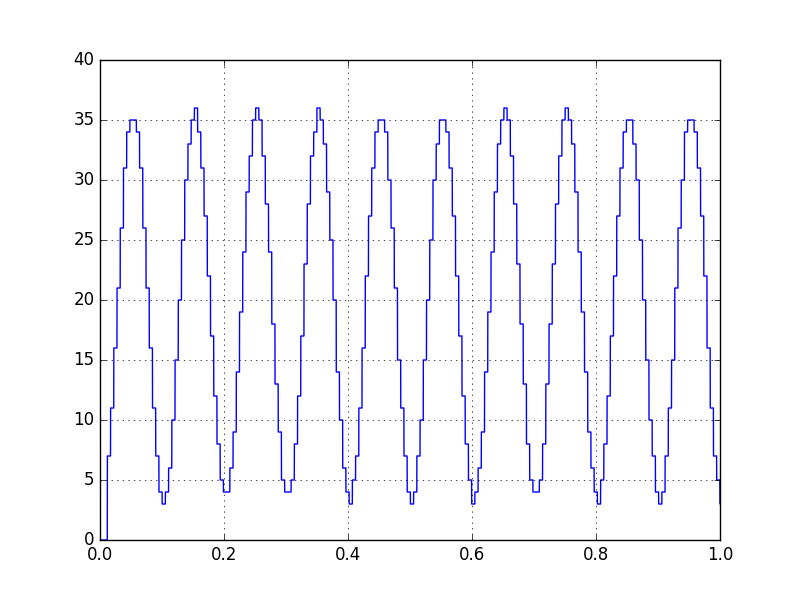
\includegraphics[width=0.4\textwidth]{figures/figure_2.png}
    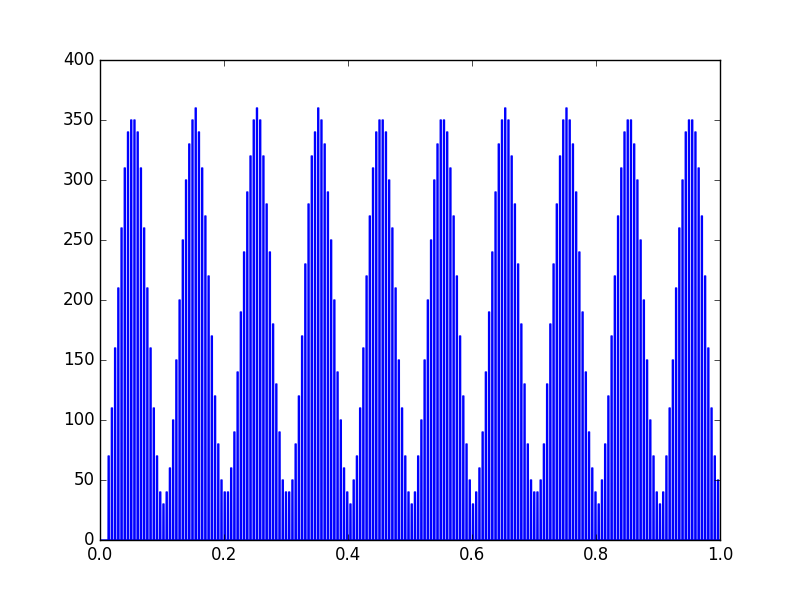
\includegraphics[width=0.4\textwidth]{figures/figure_1.png}
    \caption{Risultato della simulazione del modulo gain: input a sinistra e output a destra}
    \label{fig:results}
\end{figure*}

\section{Risultati}
In figura \ref{fig:results} \`e possibile verificare come la funzionalit\`a del gain \`e stata perfettamente implementata
sfruttando lo standard FMI. Il valore in input (nell'immagine a sinistra) viene moltiplicato per 10 come da specifica 
(immagine a destra).

\section{Conclusioni}
Il tutorial ha permesso di verificare i vantaggi introdotti dallo standard FMI, che risultano dunque concentrarsi sulla
possibilit\`a di far integrare in una piattaforma virtuale diversi componenti eterogenei, senza preoccuparsi del loro
linguaggio di definizione, per permetterne una facile simulazione.

\bibliographystyle{IEEEtran}
\bibliography{biblio}

\end{document}